In questo capitolo verrà affrontato il processo di riconoscimento delle stanze a partire dalle mappa SLAM generata attraverso i sensori LIDAR del robot. In particolare, verrà presentato il processo di individuazione proposto da \cite{mora}, le modifiche adottate e la console per poter visualizzare e modificare i risultati ottenuti.\\\\
I risultati ottenuti da questo processo verranno utilizzati per la generazione del grafo delle stanze nella mappa semantica.

\section{Riconoscimento delle Stanze}

\begin{figure}[H]
  \centering
  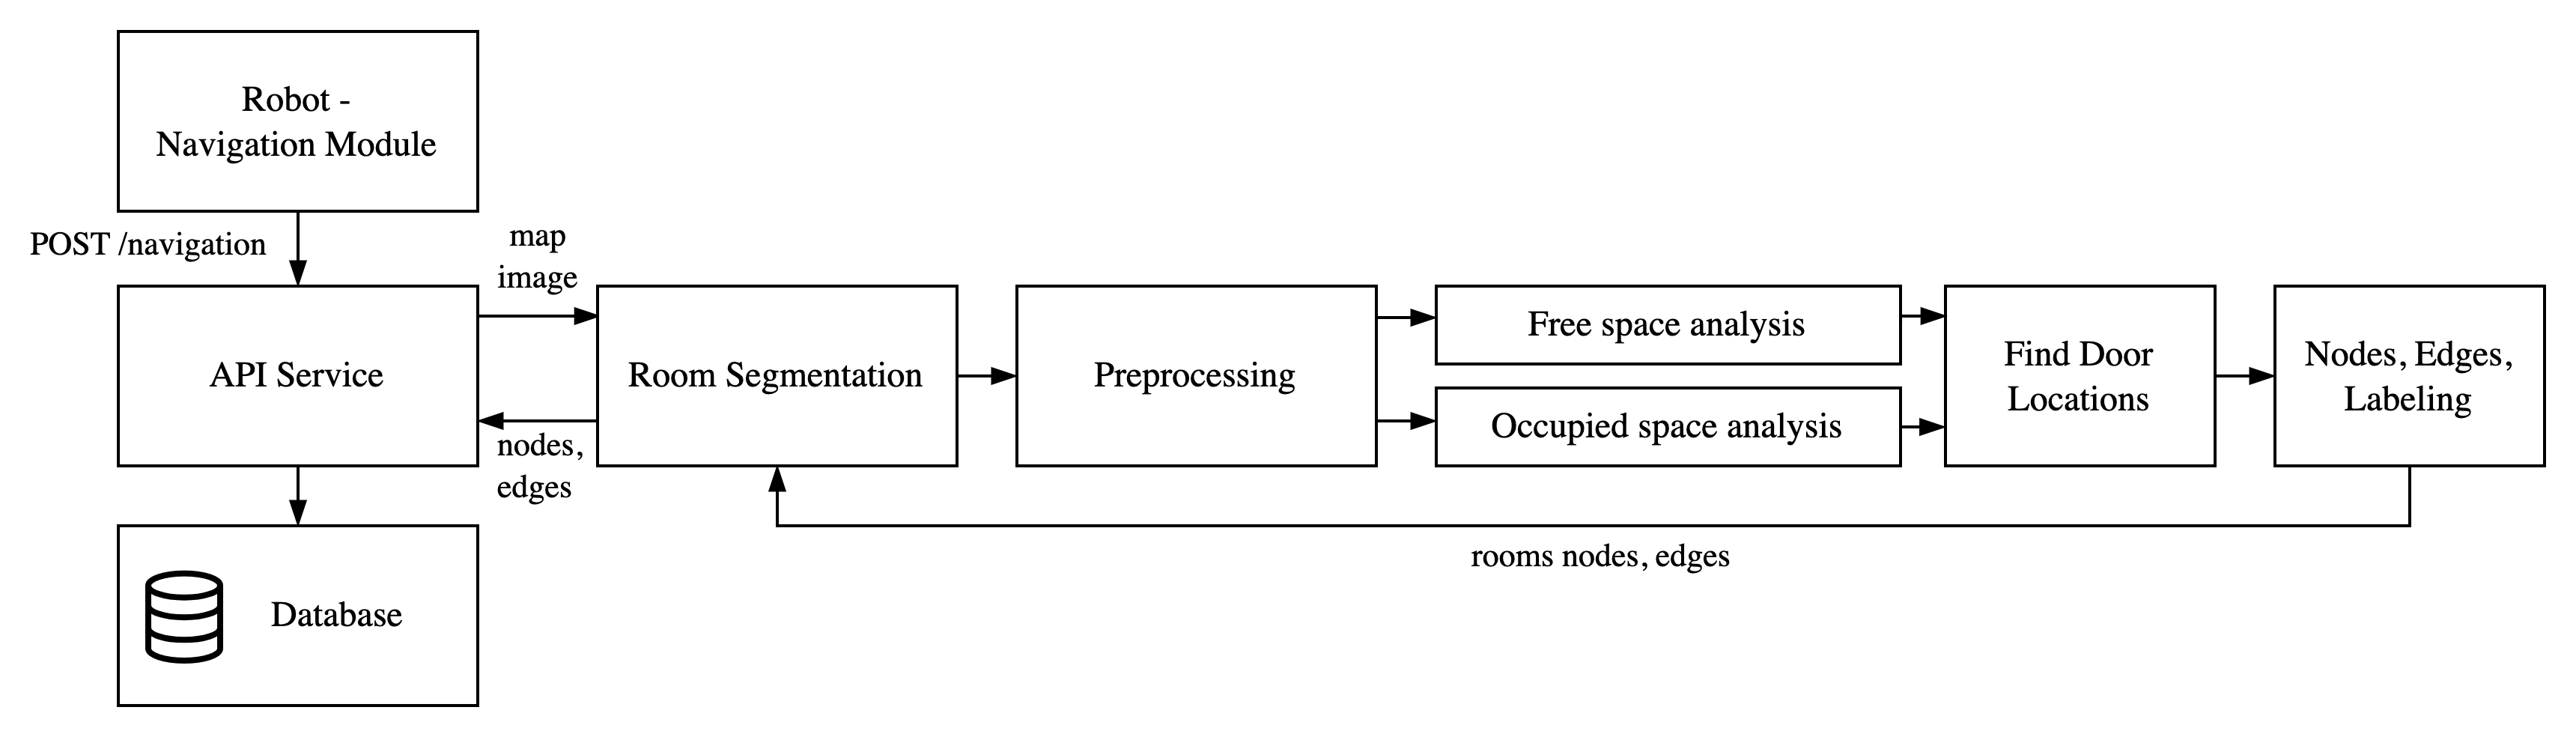
\includegraphics[width=\textwidth]{room_recogn.png}
  \caption{Schema dei flussi dati per il riconoscimento delle stanze e il salvataggio del grafo delle stanze}
\end{figure}

\subsection{Voronoi}


\section{Visualizzazione e Modifica delle Stanze}

\section{Conclusioni}